\section{The Model - Part 2}
\subsection{Data and Results}



\begin{frame}
\frametitle{Data}
The second part of the paper uses data from the Spanish Empire and Peruvian Republic to test channels of persistence. 
\begin{itemize}
    \item Land Tenure: Looking the impact of the mita on the formation of haciendas.\\[10pt]
    
    \item Public Goods: Looking the mita’s impact on education in 1876, 1940, and 2001. Also looking by the effect over roads.\\[10pt]
    
    \item Market Participation: Looking at the percentage of the district labor force whose primary occupation is agriculture, taken from the 1993 Population Census.\\[10pt]
    
\end{itemize}



\end{frame}

\begin{frame}
\frametitle{Results}

Land Tenure
\begin{itemize}
    \item Very large mita effect on the concentration of haciendas in the 17th century (robust support for a persistent impact) .\\[10pt]
    
    \item Mita lowered the percentage of the rural tributary population in haciendas in 1845 by around 20 percentage points.\\[10pt]
    
    \item  The percentage of the rural population in haciendas nearly doubled between 1845 and 1940. This expansion was spurred by a large increase in land values due to globalization and seems to have been particularly coercive inside the mita catchment.
\end{itemize}

\end{frame}


\begin{frame}
\frametitle{Results}

Public Goods
\begin{itemize}
    \item The paper find little evidence that a mita effect persists through access to schooling. Most of results were no significant.\\[15pt] 
    \item Pronounced disparities in road networks across the mita boundary.
    
\end{itemize}

\end{frame}

\begin{frame}
\frametitle{Results}
\begin{center}
    

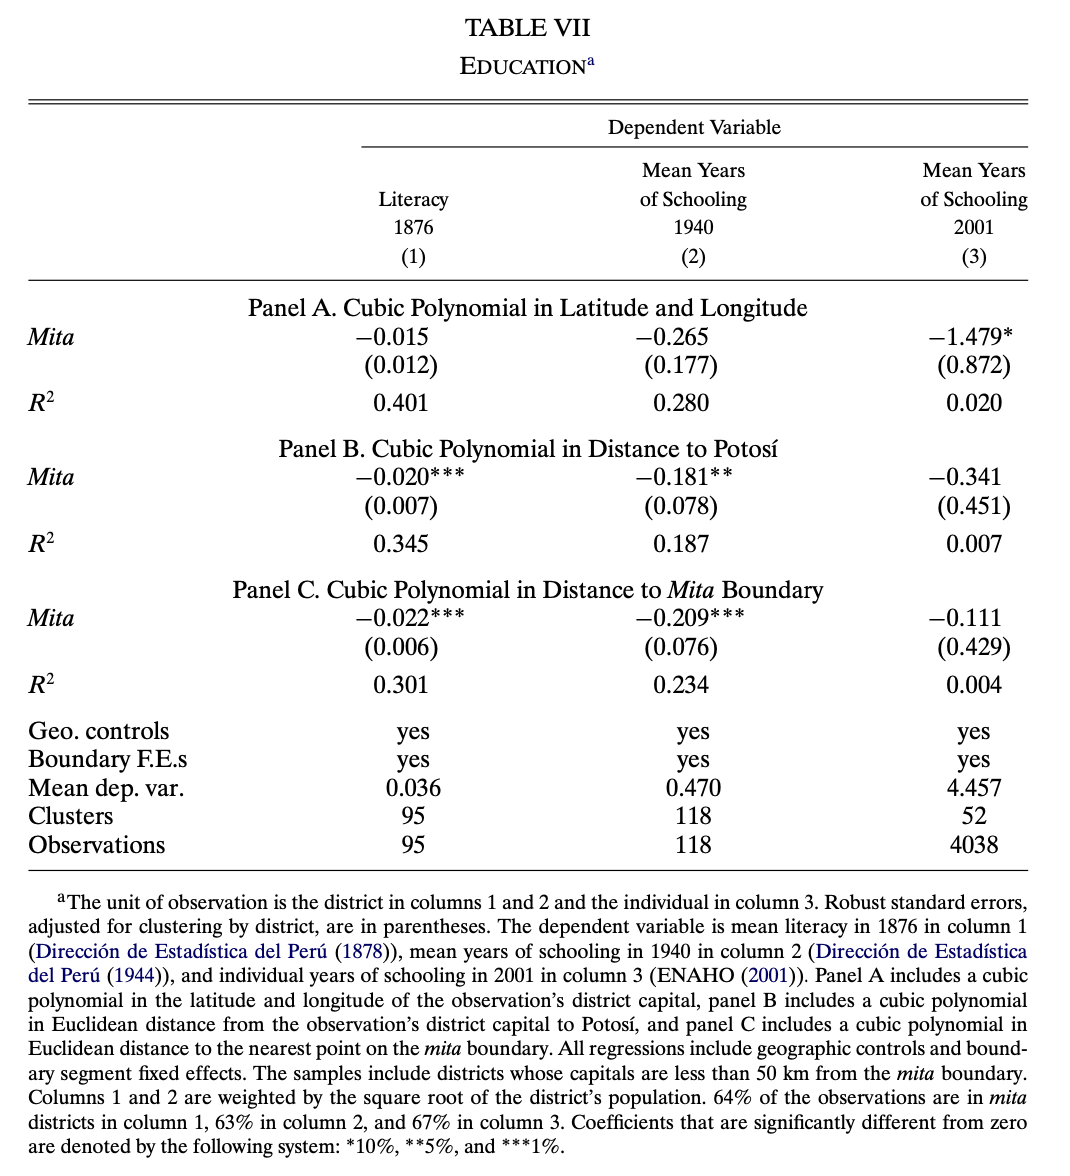
\includegraphics[width=.7\textwidth] {peru7.png}

\end{center}
\end{frame}


\begin{frame}
\frametitle{Results}

Market Participation
\begin{itemize}
    \item There are evidence that the mita’s effects persist in part through an economically meaningful impact on agricultural market participation, although the precise magnitude of this effect is difficult to convincingly establish given the properties of the data.\\[15pt]
    
    \item Most residents in mita districts are engaged in subsistence farming. This is related to the increase in transaction costs due to the early results of the effect of the mita in roads.
    
\end{itemize}

\end{frame}
\begin{frame}
\frametitle{Results}
\begin{center}
    
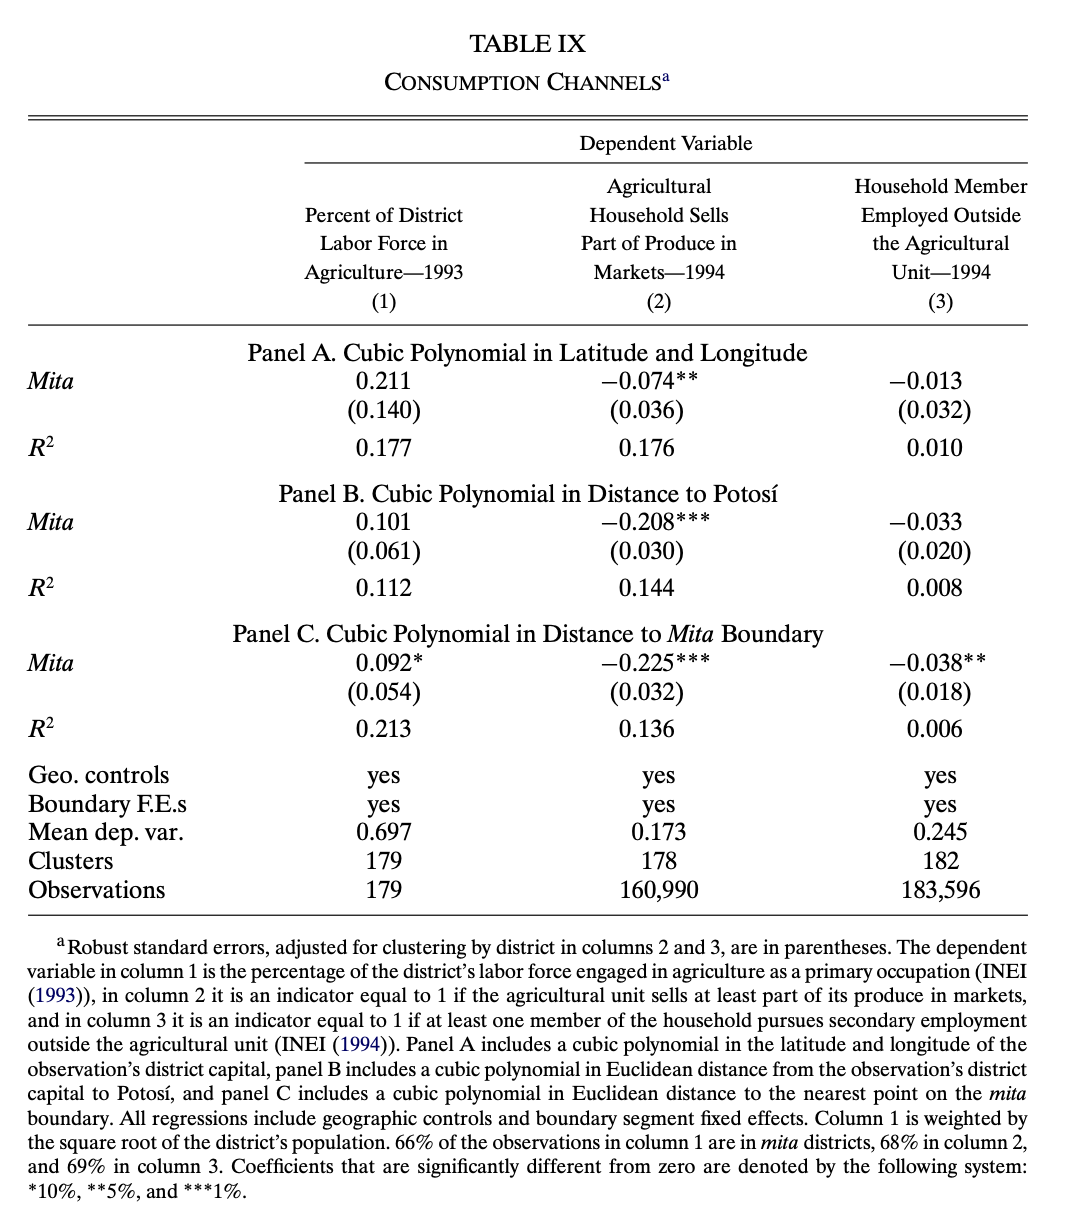
\includegraphics[width=.7\textwidth] {Peru9.png}

\end{center}
\end{frame}
